\documentclass[SoftwareDesign/SoftwareDesign_main.tex]{subfiles}

\begin{document}
\section{Design af Notifikation vinduet}
Inde i Headerbaren findes et ikon, som udfolder ved aktiveringen (Bruger interaktion). Heri præsenteres brugeren alle de notifikation, heri beskeder, som er 'nye' for ham: beskeder som han ikke tidligere har interageret med. Disse notifikation er 'nedkogt' besked, som kun indeholder de vigtigste informationer - det kunne fx være senderen og de første ord i den beskedstreng sendt. Den visuelle repræsentation af vinduet kan se i figur \ref{fig:wire_noti}. Der kan være forskellige notifikationbeskeder, og det skal være let at tilføje nye beskedtyper. Der er to type beskeder defineret indtil videre: 
\begin{enumerate}
    \item Udlejer respons til anmodning
    \item Lejer anmodning om bil
\end{enumerate}
\begin{figure}[H]
    \centering
    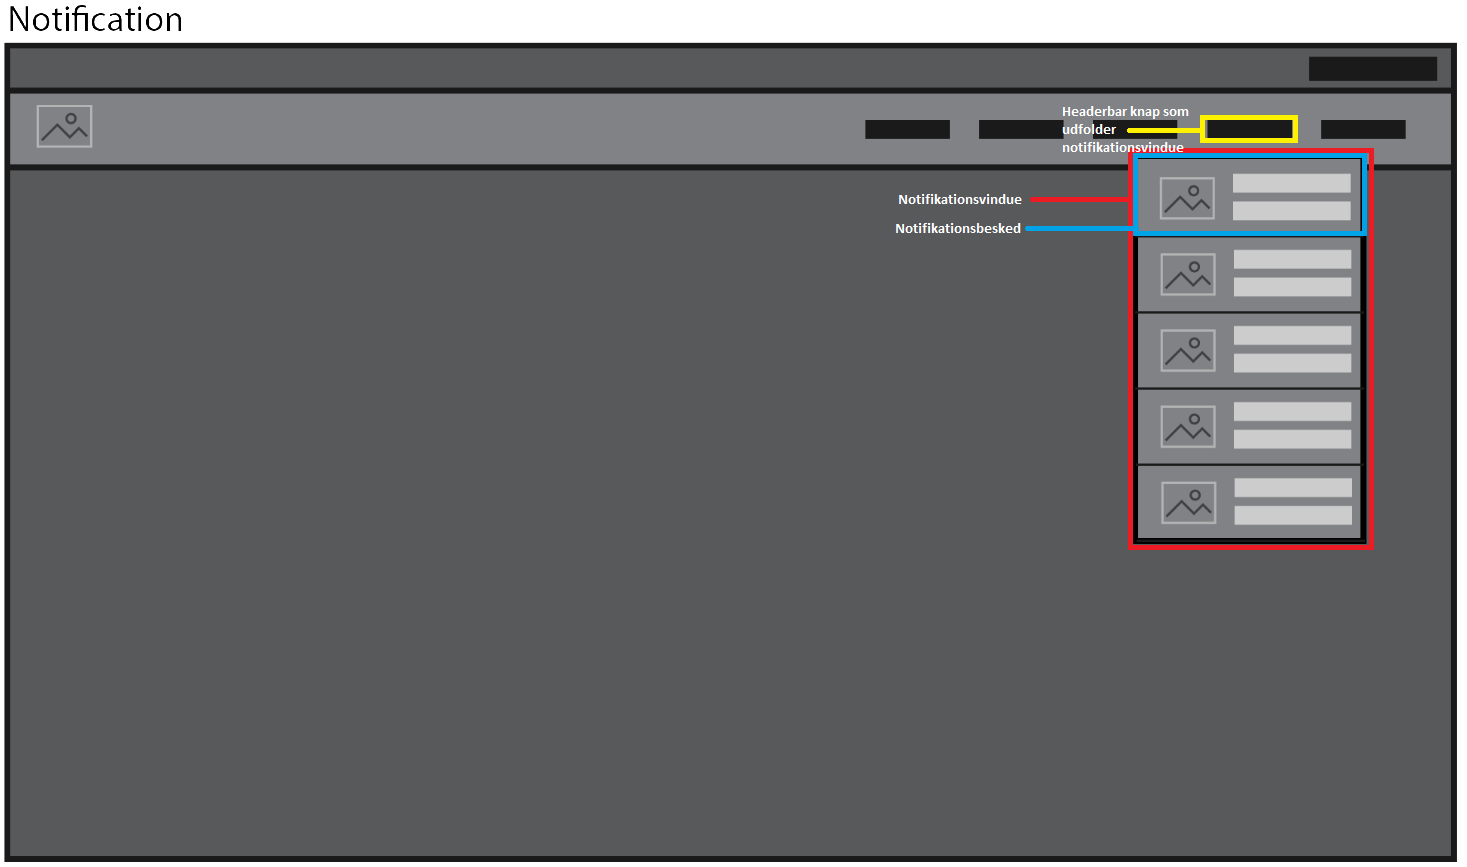
\includegraphics[width=\textwidth]{SoftwareDesign/MVVMDesigns/Graphics/noti_wirefame.png}
    \caption{Frame for Notifikations vinduet}
    \label{fig:wire_noti}
\end{figure}

\subsection{Besked opbygning}
Notifikationsvinduet skal kunne indeholder forskellige typer beskeder, og det skal være let at tilføje nye beskeder. Beskederne hentes fra databasen, hvor deres given typer definerer, hvordan de vises i notifikationsvinduet. I de følgende delafsnit forklares hvordan dette designes og figur \ref{fig:cd_noti} viser et klassediagram af operationen

\begin{figure}[H]
    \centering
    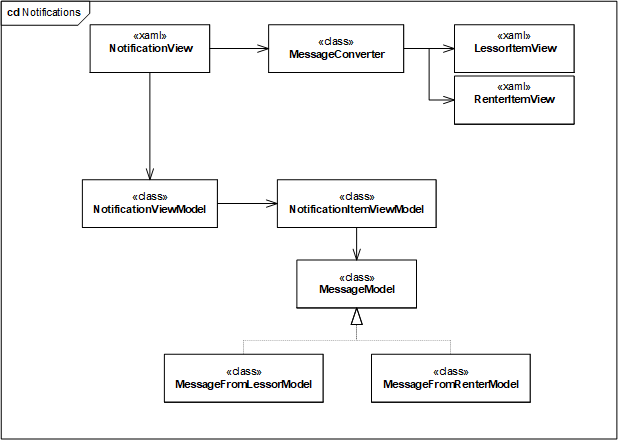
\includegraphics[width=\textwidth]{SoftwareDesign/MVVMDesigns/Graphics/cd_notification.png}
    \caption{Klassediagram for notifikationer}
    \label{fig:cd_noti}
\end{figure}

\subsection{MessageConverter}
En bruger vil modtage notifikationer, når han interagere med applikationen, fx når der enten lejes eller udlejes en bil. Disse notifikationer 'pop'er up' og vises i headerbaren. Hver type besked vises forskelligt, der skal således runtime differenceres mellem besked typerne. Hertil bruges en 'valueconverter', som konverterer en besked til et 'wpf item' i notifikationsvinduet - en notifikationsbesked, repræsenteret som en blok inde i notifikationsvinduet (Se figur \ref{fig:wire_noti}. Hvert besked har dets egen model, og for at illustrere informationer, skal der laves et tilhørende 'ItemView' for beskedmodellen - 'LessorItemView' er det visuelle vindue for informationen gemt i beskeden 'MessageFromLessorModel'. 
Hvis systemet udvides og der tilføjes flere typer beskeder, kan de let tilføjes ved at oprette et nyt ItemView, samt at beskederne nedarver fra MessageModel. 

\subsection{Interaktion med modeller og database}
For hvert gang der registreres nye beskeder for den specifikke bruger fra databasen, opdateres notifikationsvinduet. Når notifikationsvinduet aktiveres, vil det altid vise alle ulæste beskeder - når brugeren trykker på en notifikationsbesked, navigeres han til et andet vindue, som viser hele beskedens indhold, notifikationsbeskeden fjernes herefter fra notifikationsvinduet. 
\end{document}